\documentclass{fkssolpub}

\usepackage[czech]{babel}
\usepackage{fontspec}
\usepackage{fkssugar}
\usepackage{amsmath}
\usepackage{graphicx}

\author{Ondřej Sedláček}
\school{Gymnázium Oty Pavla} 
\series{3p}
\problem{5} 

\begin{document} 

\begin{figure}[h!]
  \centering
  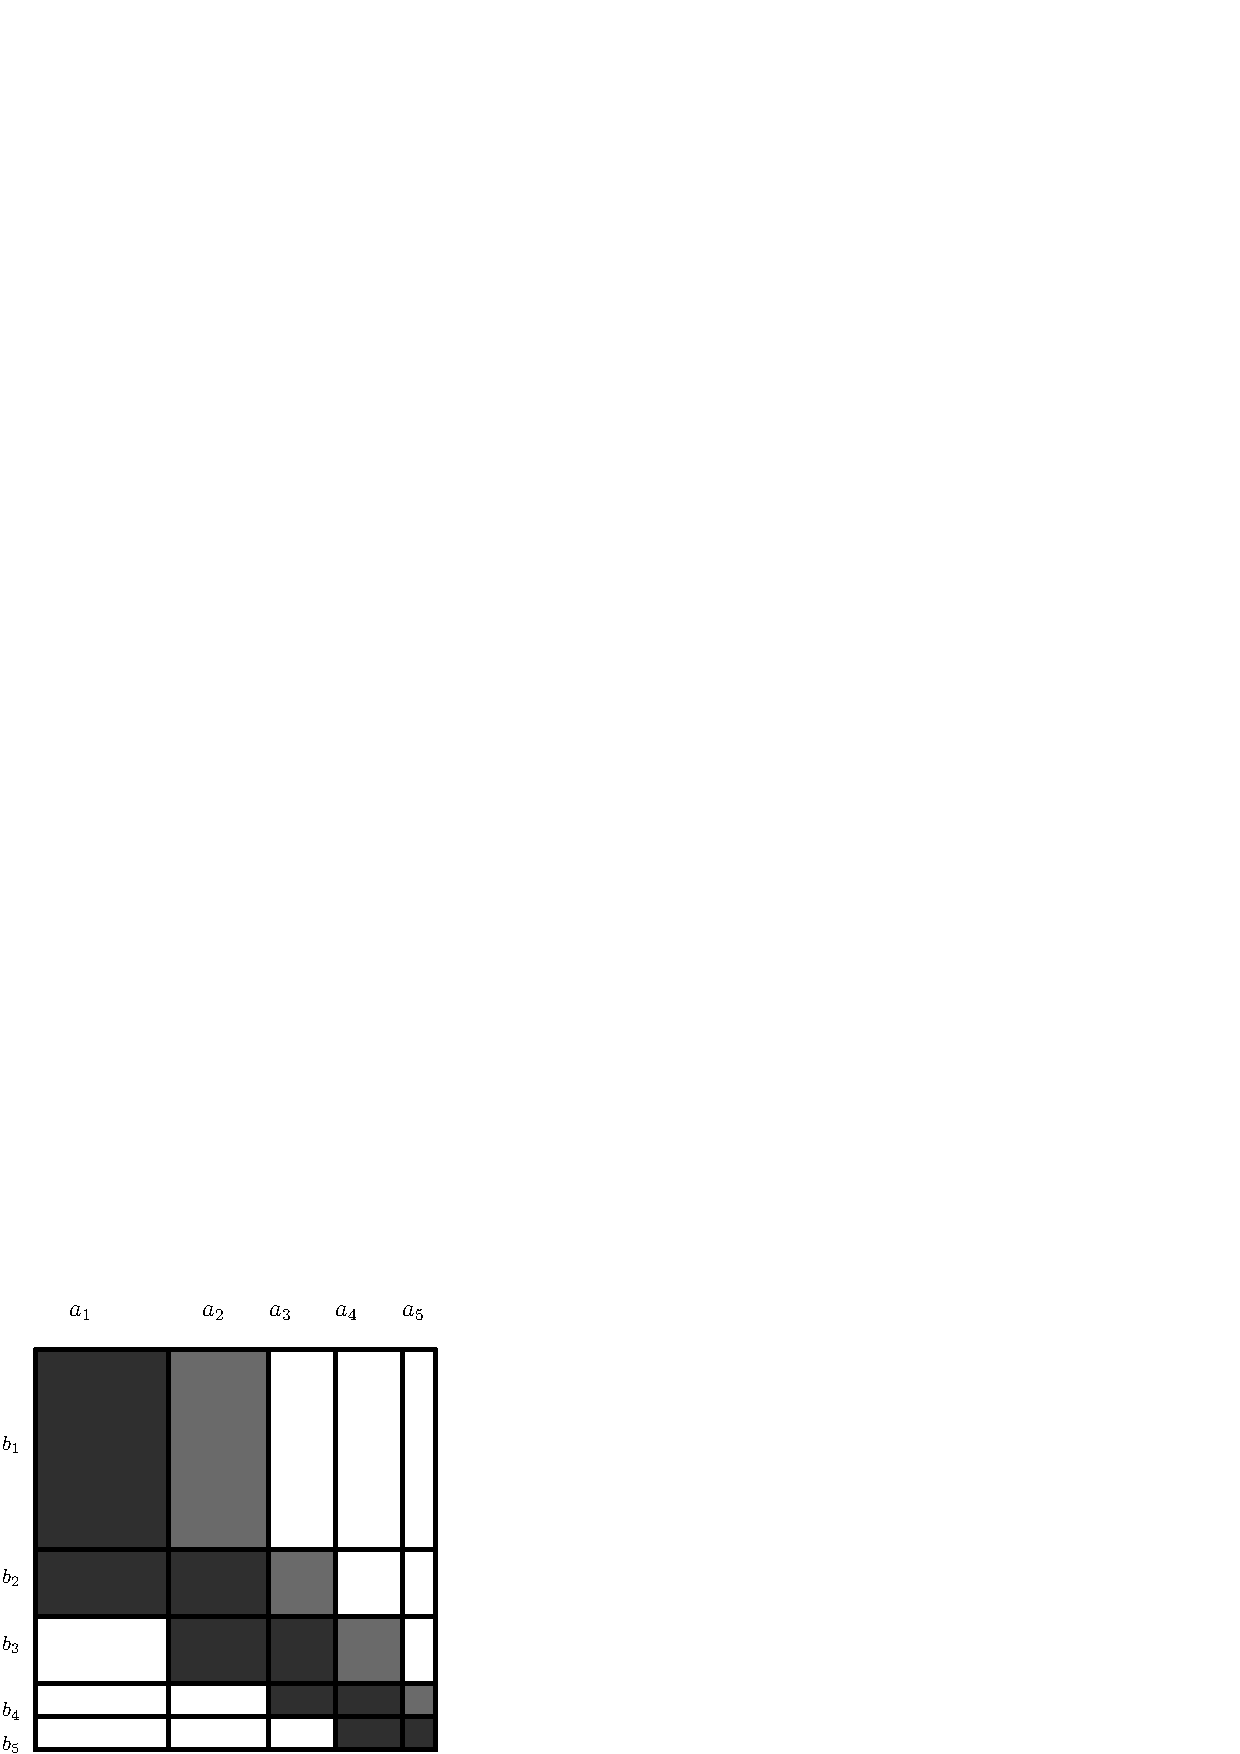
\includegraphics{5-fig.png}
  \caption{Konstrukce ze zadání s doplněnými úhly}
\end{figure}

Abychom dokázali výrok ze zadání, uvědomím si, že pokud průměr kružnice opsané ABH
bude roven poloměru kružnice $k$, pak se kružnice opsaná ABH dotýká kružnice $k$. 
To platí díky tomu, že pokud průměr
té kružnice opsané splňuje tuto podmínku, právě jeden bod té kružnice opsané,
ten nejvzdálenější, bude vzdálen od bodu H o poloměr kružnice $k$, tím pádem bude
ležet i na kružnici $k$.

Nechť $|\angle BDA| = |\angle DBC| = \gamma$. Abychom zjistili velikost úhlu $\angle
BHA$, nejprve půjdeme přes pravý úhel mezi výškou na stranu AD a stranou BC, pak
dopočítáme úhly v pravoúhlém trojúhelníku BEH a následně dopočítáme $|\angle BHA|
= 180^{\circ} - \gamma$.

Následně dopočítáme velikost úhlu $\angle DHC$ jednoduše tím, že čtyřúhelník
HBCD je tětivový díky pravým úhlům u vrcholů B a D. Odtud pak $|\angle DHC| = \gamma$.

Teď už nám zbývá ukázat, že poloměr kružnice $k$ a průměr kružnice opsané
trojúhelníku ABH je stejně velký. Protože trojúhelník CDH je pravoúhlý s
přeponou CH, zjištěním poloměru jeho kružnice opsané získáme velikost poloviny
úsečky CH, která má stejnou velikost jako poloměr kružnice $k$. Pomocí sinové
věty formulujeme vztahy:

\[
  2r_{ABH} = \frac{|AB|}{\sin (180^{\circ} - \gamma)}
\]
\[
  2r_{CDH} = \frac{|CD|}{\sin \gamma}
\]

Protože $|AB| = |CD|$ a $\sin \gamma = \sin (180^{\circ} - \gamma)$, jsou si poloměry
těchto kružnic rovny. Z toho vyplývá, že průměr kružnice opsané trojúhelníku ABH je
roven poloměru kružnici $k$. Q. E. D.

\end{document}
